\chapter{Design of a Flexible Visual Debugging System/Tool/Framework?}
\label{visual_debugging_system}

Debugging in robotics has unique requirements which are often not met by traditional debugging systems. The special requirements lead to a number of different tools to support debugging in robotics. The previous chapter summarized some of those tools and issues of existing solutions were identified: a) The tools either focus on visualization of pre-defined spatial data or render data as text messages. b) The graphical interfaces are rather static and difficult to adapt to different usage scenarios.

This chapter introduces a new system for debugging in robotics, tailored to tackle the challanges developers face when debugging robotic systems. The first section states the hypothesis behind the ideas that have driven the development of the debugging system. Section two will state the goals of the work, which leads to specific requirements for this system. The system design section presents the design for a flexible visual debugging system.

[----> where should I introduce the word dashboard and widget? goals? user interface?]

%Write about the general requirements for a visual debugging system, rosdashboard would be one possible implementation. This basically could explain most of rosdashboard, apart from the ros specific part which is: topic subscription setup (gui), topic introspection to wait for message class types, topic subscription (code) and calling the value update hook. Saving to file saves the topic configuration which is ros specific as well.

%Point out that ROS was targeted early on and affected many decisions, but the requirements and the system design is applicable in general. [Andreas: not sure if this is the right place, might be better in the introduction, since it explains the dominance of ROS tools in related work / debugging in robotics]

%--> Generalize design decisions, if they apply for other robot frameworks as well.

%%%% HYPOTHESIS %%%%
\section{Hypothesis}
A possible reason why many developers still use print or logging statments to debug their programs is because these methods can be immideately used when required. Developers don't need to undergo a lenghty setup and configuration process before they can start debugging and they don't need to gain extensive knowledge about the methodology and tools either. The overhead to set up and configure a debugging system should be reduced to make the system easy to use without extensive knowledge about the debugging methodology and tool.

The main issue with print or logging statements is the text-only representation of data. The system proposed in this chapter aims to support the developer during debugging by visualizing data in a graphic way and thus eliminating the cognitive effort needed to parse and interpret text based logging messages. The cognitive effort required during debugging can be further reduced by a flexible system which can be adapted to different preferences of different developers. Every developer can choose a visualization that fits their mental model of the debugged data best.


%%%% GOALS %%%%
\section{Goals}
The main goal of this work is to design a debugging system which is suitable for debugging in robotics and can be used to evaluate the hypothesis stated above. The design of the system is independent of a specific robotic framework and could be implemented for any available framework.
While most of the currently available visualization tools in robotics focus on pre-defined and spatial data to help understand the robot and the environment in which it runs \cite{Collett2010, Quigley2009}, rendering of abstract data is still uncommon. The design of the debugging system should be flexible enough to allow visualization of arbitrary and abstract data. Although abstract data will be the main focus of the debugging system since tools to visualize pre-defined data are already widely available, the designed system is not restricted to abstract data.

The system provides a graphical user interface which can be used by developers to visualize all kinds of data from the robotic application. The developers can customize the visualization according to the current robot hardware, development stage and personal preferences. The system can be adapted to many different use cases and should reduce the cognitive effort during debugging by visualizing the data according to the mental model of the developer and meaning of the data.

%%%% REQUIREMENTS %%%%
\section{Requirements}
The requirements of the flexible visual debugging system are mostly dominated by the special requirements of robotics. Some requirements are derived from the hypothesis and focus more on development performance and speed. This section presents the elicited requirements for a flexible visual debugging system.

\subsection{Distributed Live Debugging}
When debugging robotic applications it is usually not possible to interrupt the execution of the application and follow a step-through approach. All data must be captured, processed and visualized live. Robotic applications are usually distributed systems, because they often run on mobile robots or are so complex that multiple computers are used to make the system faster. This means the system must be able to handle communication distributed across a network.

\subsection{Adaptable Tool}
Due to many different application scenarios in robotics and the diverse environment of available frameworks for robot development, many researchers and developers have built their own tools to support them during debugging \cite{Collett2010}. Developing your own debugging tool is extremely time consuming and the developed tools are often one-time-only tools, because they don't fit the use case of other applications and are too hard to adapt to a new project.
In order to allow the use of the proposed debugging system in many different scenarios and use cases, flexibility has a high priority. Flexibility not only means the system can be adapted easily to fit different problems, it also means the system can be adapted to suit different developer's preferences. Each developer might prefer a different kind of visualization of the collected data, thus loose coupling of the collected data and the visualization widgets is necessary.

\subsection{Low Configuration Overhead}
Iterative development, small changes are deployed during development, setting up must be fast and easy and should not distract from the problem analysis task.

Debugging robotic applications is a highly iterative process, where small changes are made and immediately deployed to the robot. The debugging system should keep the configuration overhead as minimal as possible so that the developer is not distracted from the problem analysis task. Adding and removing new visualizations should not require many steps, otherwise the developer will be distracted by the configuration task.

[I'm talking about adding and removing visualizations but I haven't talked about the whole dashboard principle yet. Maybe I should add that to the goals?]

%%%% SYSTEM DESIGN %%%%
\section{System Design}
Discuss architecture and how it interacts with an eventual robot framework. All of them probably have some sort of inter process communication or a communication middleware in general, which can be accessed by the visualization tool.

\subsection{Computation Model / Architecture}
How ROS was used to achieve decoupled monitoring of data (topics)?

--> this would need to be separated from ros, but probably a general strategy for decoupling the collection and visualization of data can be found (worst case: listener thread?)

\subsection{Object Model}
As in the ICRA paper. Maybe some classes should be renamed to be more ROS unspecific (like Subscription).

\subsection{API}
ROSDashboard API, think about where to talk alternatives: extend ros logging framework, use tracepoints, etc.

--> too implementation specific, this is all ROS code. I don't know if this could be done in other frameworks as well (since I don't know them really), but in theory it should be possible to create a set of helper methods for every framework that uses the built in communication layer to have one-liner publish statements.

\subsection{Graphical User Interface}
The user interface for the debugging tool should allow to add and remove visualizations easily and arrange them however the developer wants. Thus a central dashboard approach was chosen, where visualizations can be positioned freely in form of widgets. Adding new visualizations to the dashboard can be done through a "Drag \& Drop" mechanism, once the widget is on the dashboard it can be resized and repositioned on the canvas. The initial mockup of the proposed graphical user interface is shown in figure~\ref{gui_mockup}.

\begin{figure}[htbp]
  \centering
  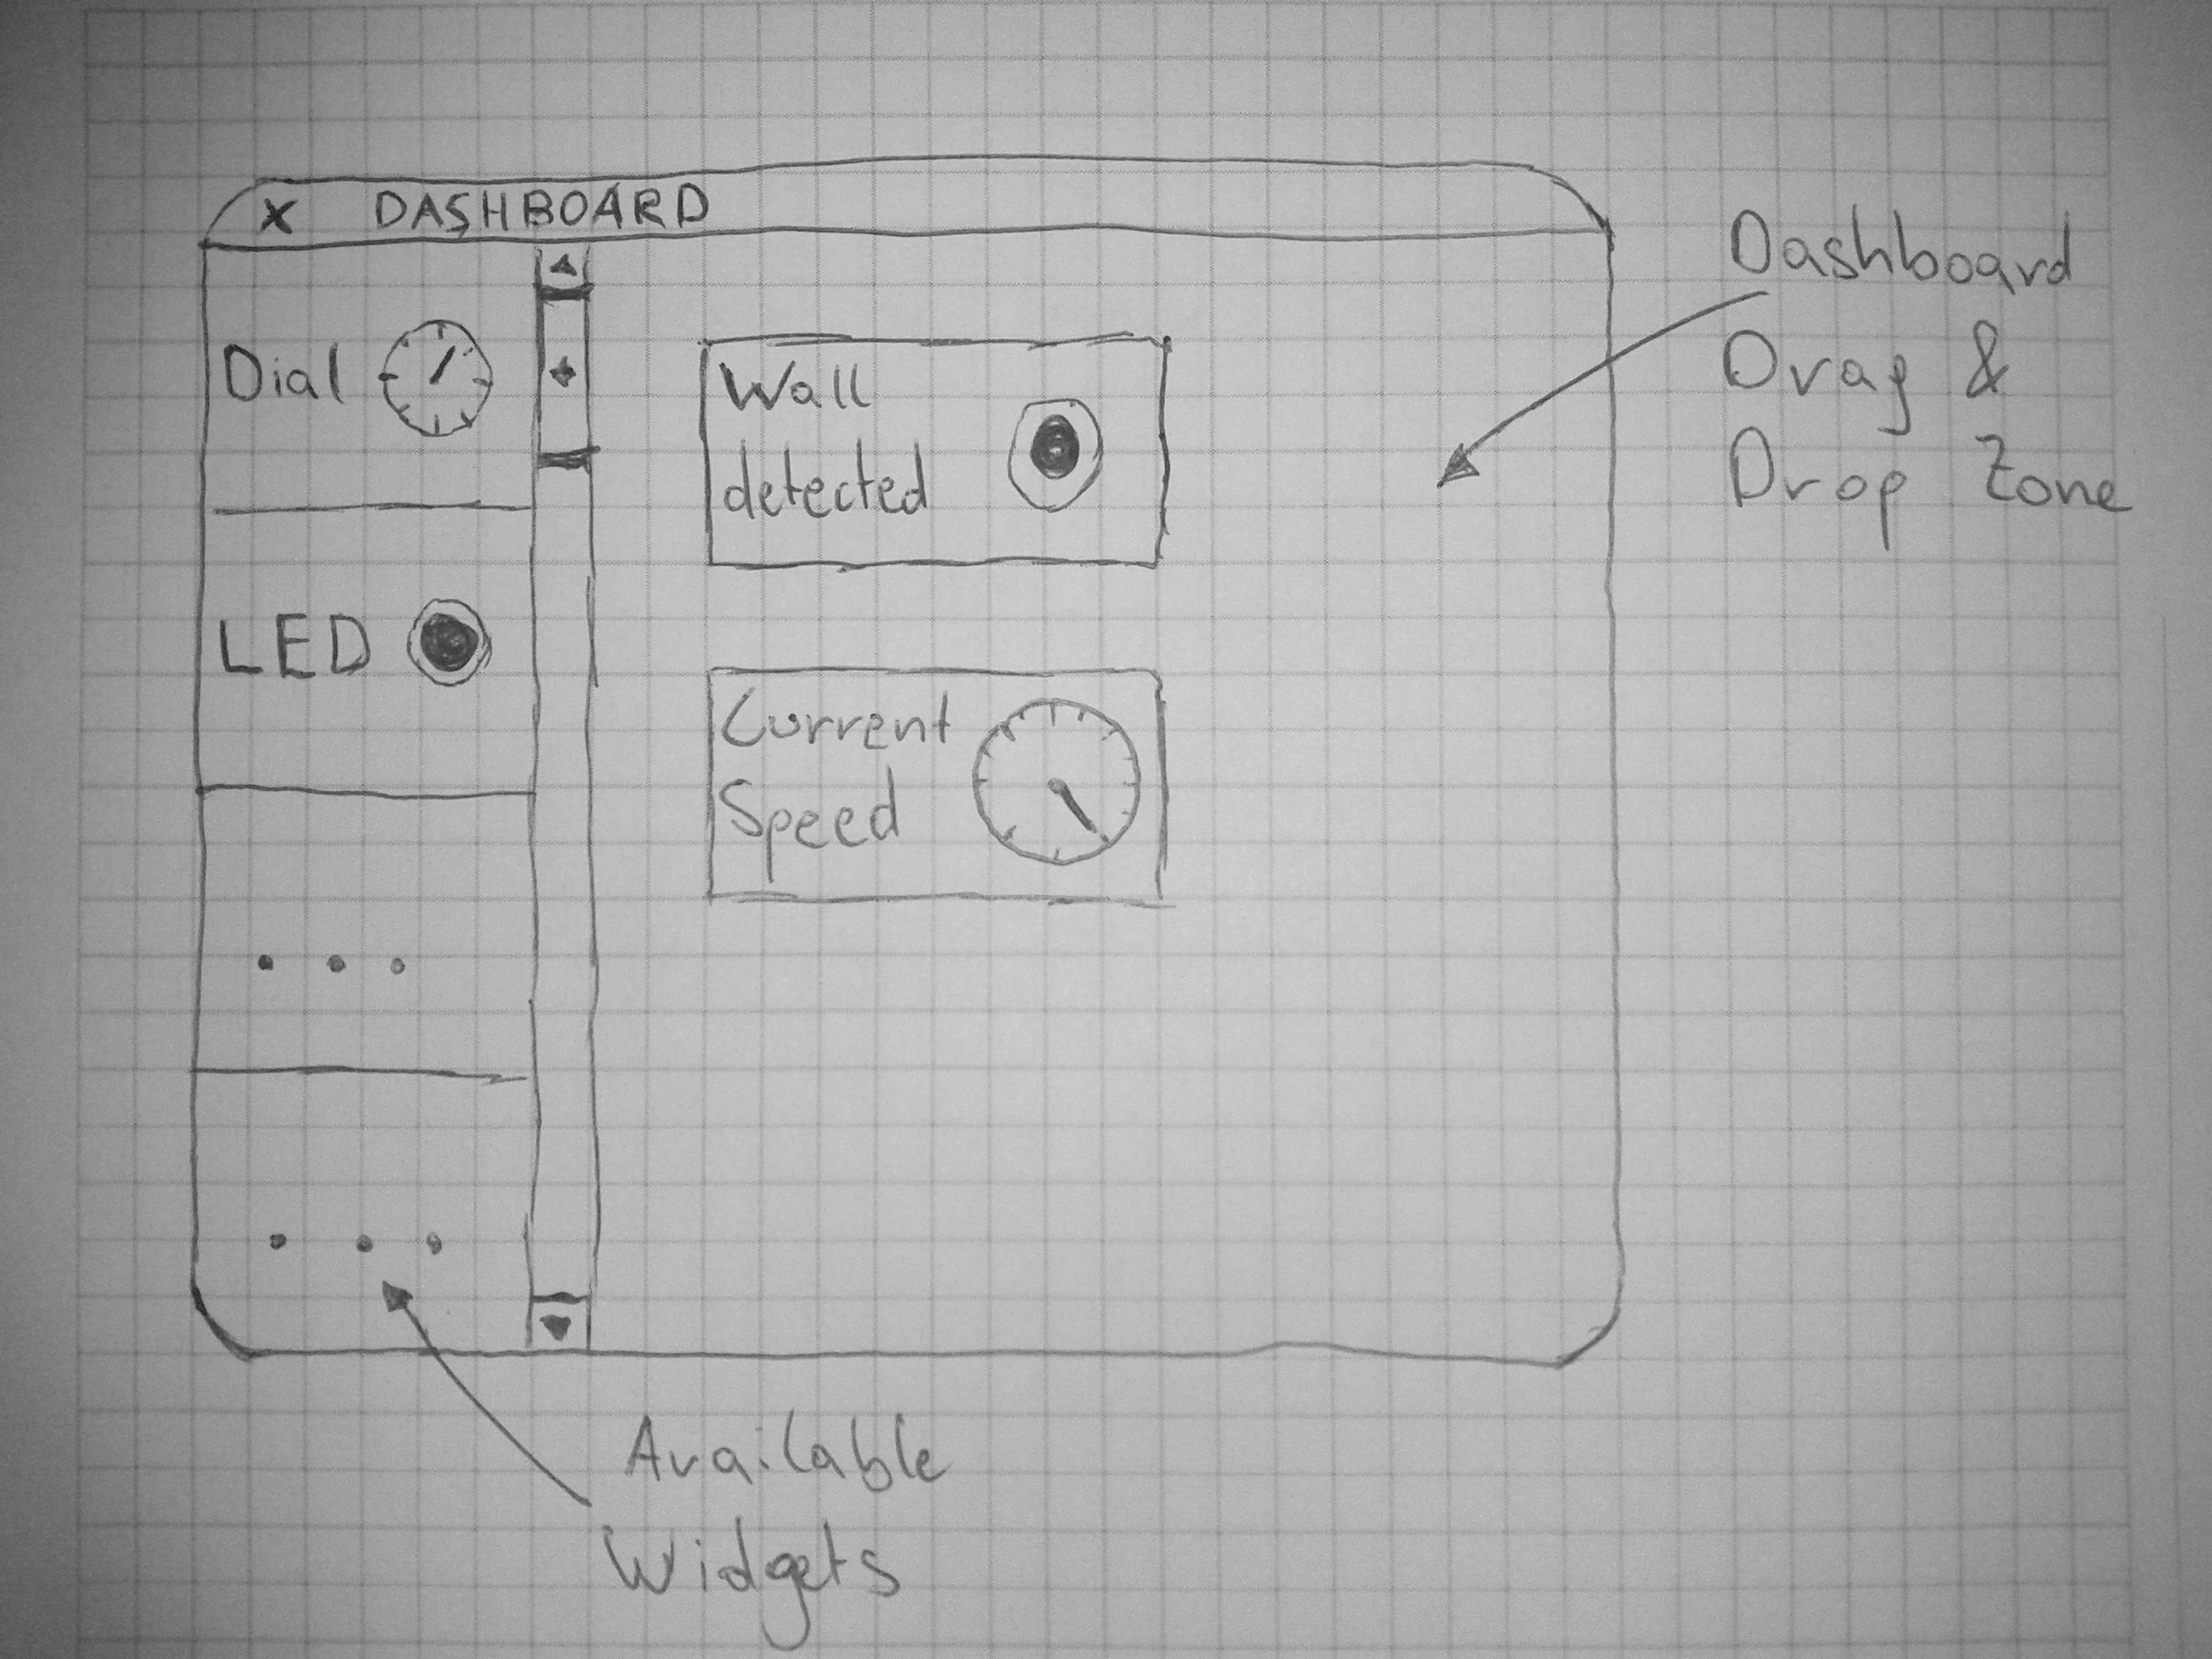
\includegraphics[width=\textwidth]{img/initial_gui_mockup.jpg}
  \caption{Paper mockup for the graphical interface.}
  \label{gui_mockup}
\end{figure}

Each widget represents one type of visiualization, this can be as simple as a dial for numberic values or more complex visualizations for more concrete data like a map visualization. Although the design of the user interface does not restrict the types of visualizations, it is intended for simple data, since other tools like RViz (see~\ref{rviz}) are more specialized for those use cases.

\begin{figure}[htbp]
  \centering
  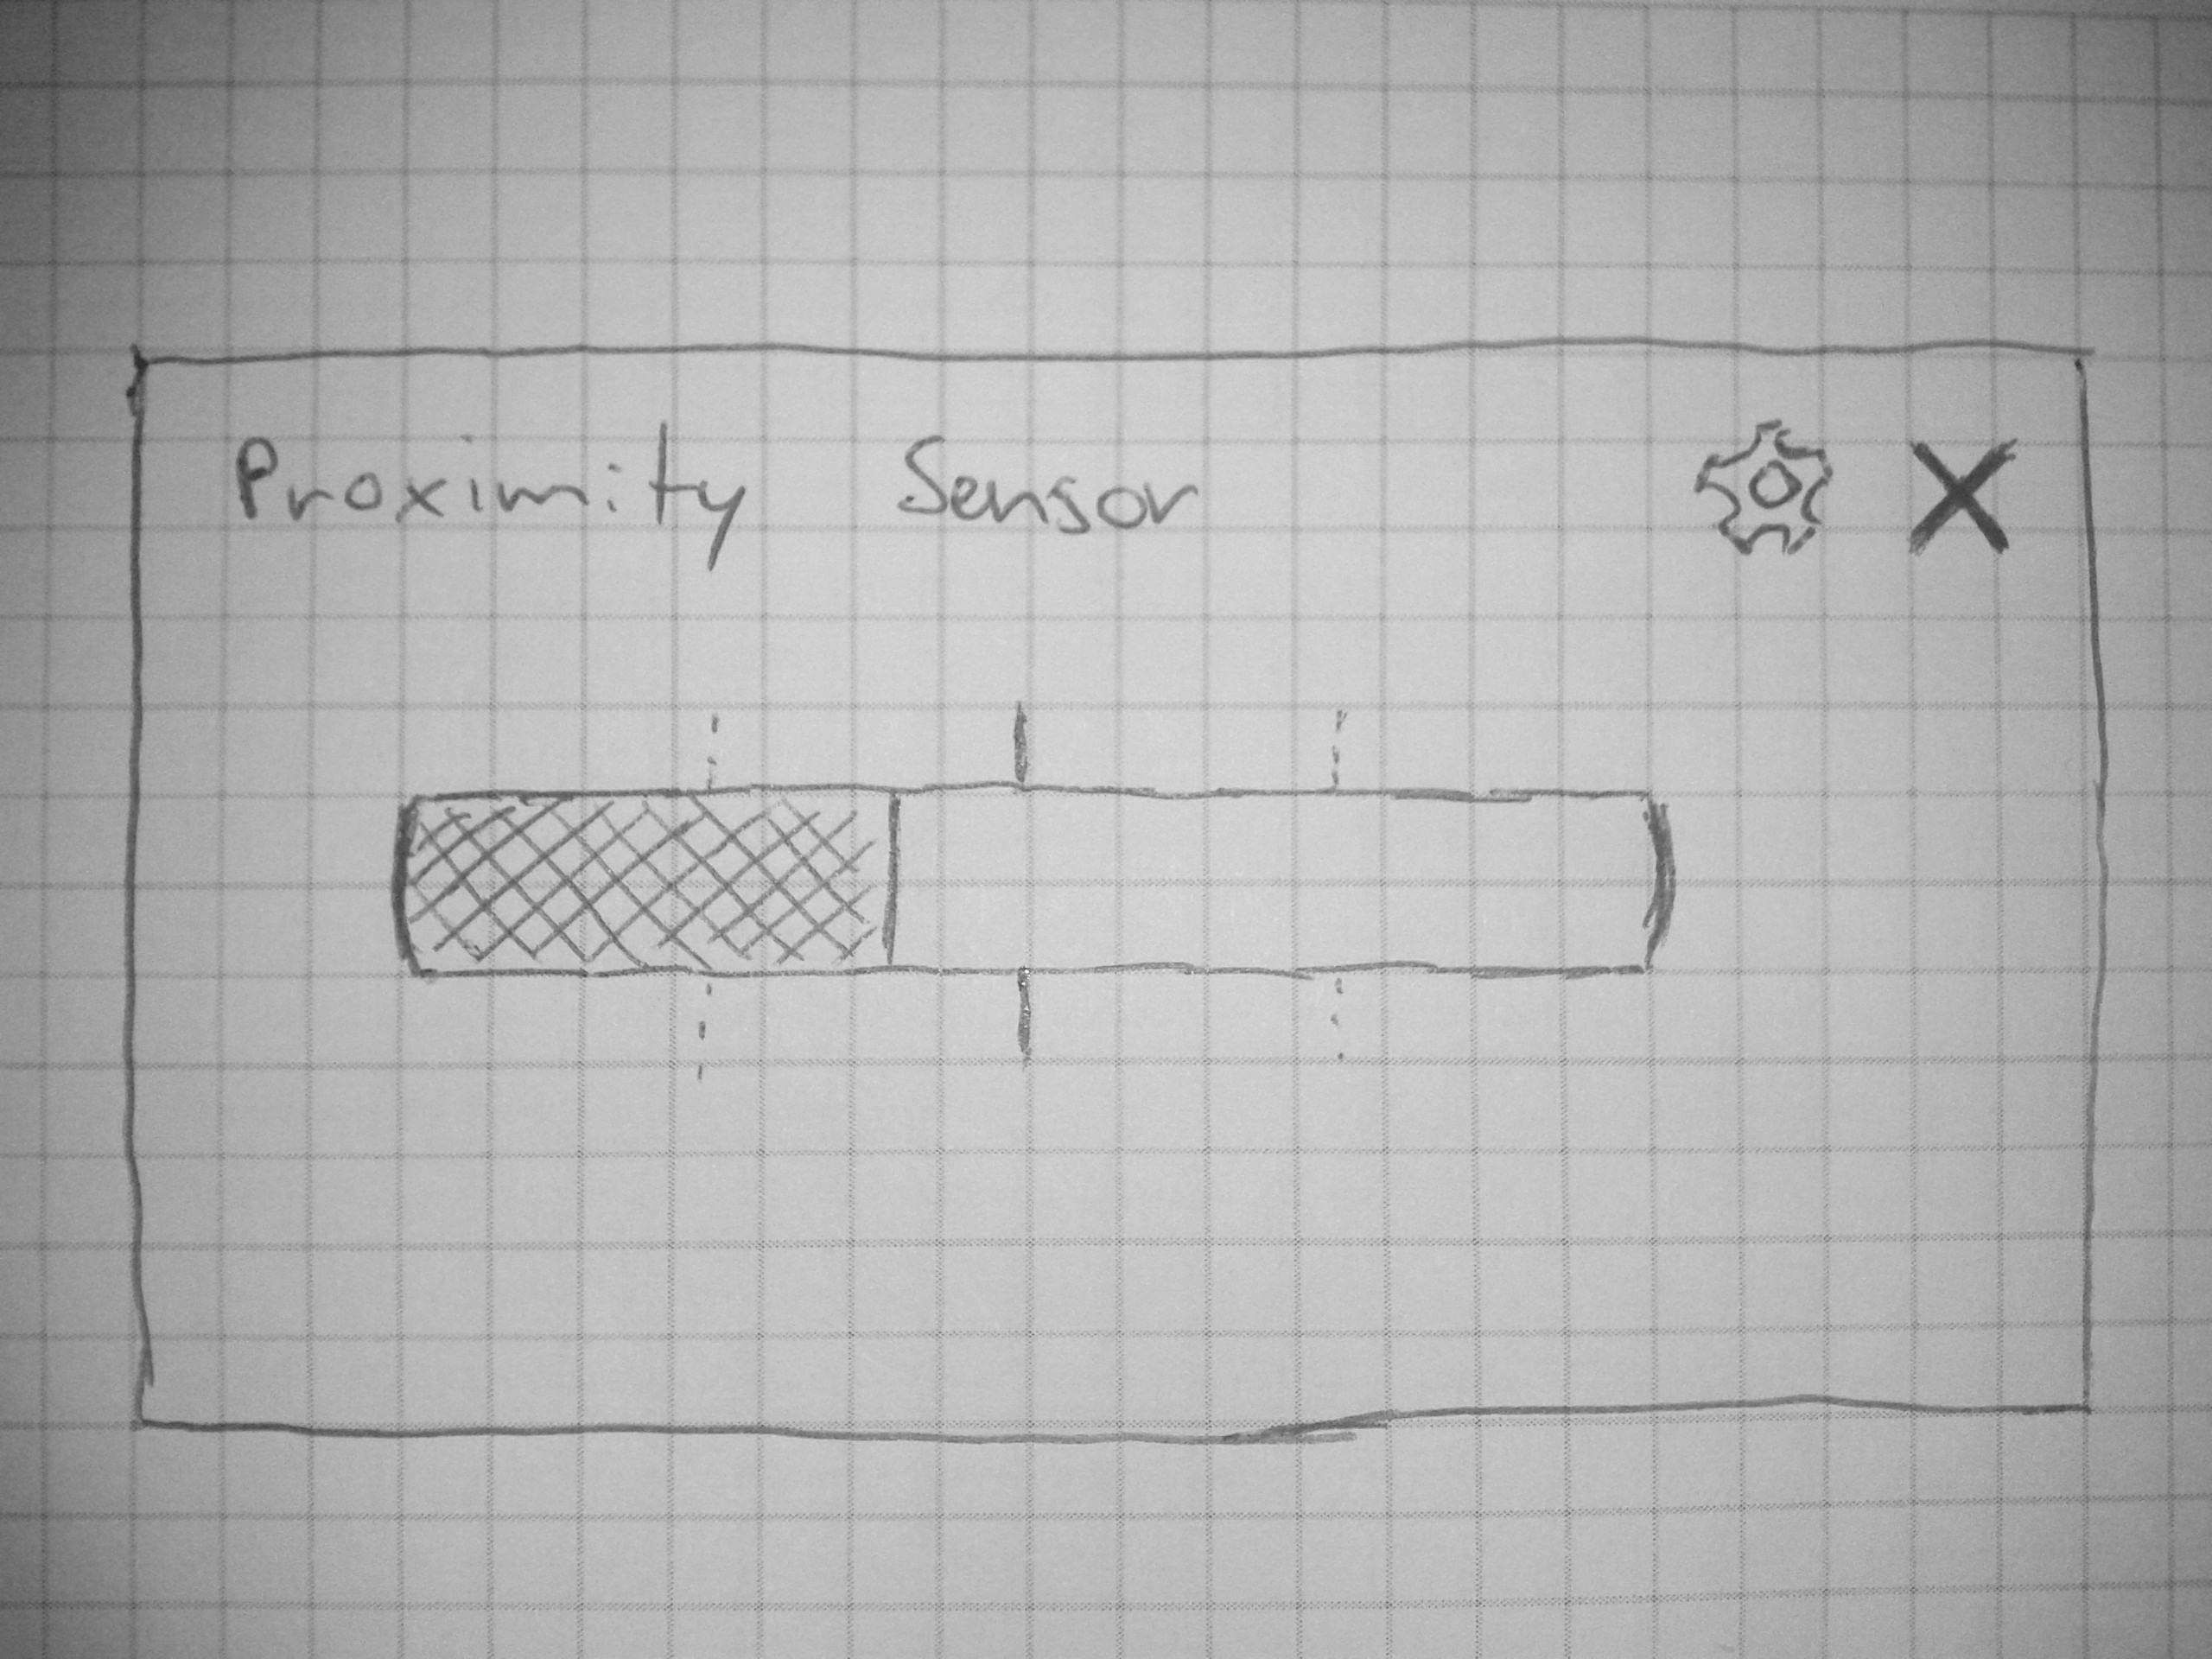
\includegraphics[width=.5\textwidth]{img/initial_widget_mockup.jpg}
  \caption{Paper mockup for a visualization widget.}
  \label{widget_mockup}
\end{figure}

Figure~\ref{widget_mockup} shows an early mockup of a widget on the dashboard. This exemplary visualization widget has the form of a progress bar where numeric values can be visualized.
